\documentclass[11pt,a4paper]{article}
\usepackage[a4paper,margin=23mm]{geometry}
\usepackage[T1]{fontenc}
\usepackage{tgpagella}
\usepackage{tgheros}
\usepackage[scaled=0.80]{DejaVuSansMono}
\usepackage{microtype}
\usepackage{graphicx}
\usepackage{amsmath}
\usepackage{xcolor}
\usepackage{listings}
\usepackage{caption}
\usepackage{float}
\usepackage{booktabs}
\usepackage{pdfpages}
\usepackage{tikz}
\usepackage{titlesec}
\usepackage[colorlinks=true,linkcolor=blue!45!black,urlcolor=blue!55!black]{hyperref}

\definecolor{navy}{HTML}{173B57}
\definecolor{blue}{HTML}{2F6F9F}
\definecolor{orange}{HTML}{D66A1F}
\definecolor{soft}{HTML}{F2F5F7}
\definecolor{codegreen}{HTML}{39754A}
\titleformat{\section}{\Large\bfseries\sffamily\color{navy}}{\thesection}{0.7em}{}
\titleformat{\subsection}{\large\bfseries\sffamily\color{blue}}{\thesubsection}{0.7em}{}
\titlespacing*{\section}{0pt}{2.2ex plus 0.5ex}{1.0ex}
\titlespacing*{\subsection}{0pt}{1.8ex plus 0.4ex}{0.7ex}
\pagestyle{plain}
\lstdefinestyle{cstyle}{
  language=C,basicstyle=\ttfamily\fontsize{8}{8.5}\selectfont,
  keywordstyle=\color{blue}\bfseries,
  commentstyle=\color{codegreen}\itshape,stringstyle=\color{orange},
  numbers=left,numberstyle=\tiny\color{gray},numbersep=7pt,
  frame=single,rulecolor=\color{black!15},backgroundcolor=\color{soft},
  breaklines=true,showstringspaces=false,tabsize=2,columns=fullflexible
}
\lstset{style=cstyle}

\begin{document}
\includepdf[pages=1,pagecommand={
  \thispagestyle{empty}
  \begin{tikzpicture}[remember picture,overlay]
    \node[anchor=center,font=\sffamily\fontsize{12}{18}\selectfont,align=left]
      at ([yshift=-67mm]current page.center) {
      \begin{tabular}{rl}
        Name: & Zhanyu Zhang \\
        UoG ID: & 2959456 \\
        UESTC ID: & 2023300901013
      \end{tabular}};
  \end{tikzpicture}
}]{../LAB 3.pdf}
\setcounter{page}{1}

\begin{abstract}
This laboratory implements task scheduling, inter-task communication, and stack allocation using CMSIS-RTOS2. The first application assigns a higher priority to a button-controlled brake indicator than to its UART notification. The second application uses two tasks and three queues to process eleven-character commands, control an LED, count toggles, and report the maximum of 150 random integers. Hardware tests confirmed the button response, command echo, and queue updates. Mean LED toggle intervals were 1006.0, 502.9, and 251.4 ms for commands of 1000, 500, and 250 ms, respectively.
\end{abstract}

\section{Introduction}
An RTOS schedules concurrent tasks according to their priorities and ready states. Thread flags communicate events, while message queues transfer values between tasks. Each task also requires a stack sized for its local data and function calls. These mechanisms are examined through a brake indication task and a UART-controlled LED task. The RTOS tick is 1 ms, and TIM4 provides a separate HAL time base.

\section{Task 1: Brake Indication and UART Notification}
Pressing B1 generates a falling-edge interrupt. The callback applies a 30 ms debounce interval and sets the brake task's thread flag. The brake task switches LD2 on, then signals the message task to transmit \texttt{Car is slowing down}. It checks for button release every 10 ms and switches LD2 off when B1 is released.

\begin{table}[H]
\centering
\caption{Task 1 priorities and stack allocation.}
\begin{tabular}{@{}llrl@{}}
\toprule
Task & CMSIS priority & Stack (bytes) & Function \\
\midrule
Brake & High & 512 & Apply the brake indicator \\
Message & Normal & 768 & Transmit the notification \\
\bottomrule
\end{tabular}
\end{table}

Brake actuation has higher priority because it is the immediate response to the slowdown signal. The LED is set before the UART task is notified. Once the brake task blocks during its release check, the message task can transmit. Both tasks wait on flags between events.

The hardware test showed LD2 illuminated while B1 was held and extinguished after release. Figure~\ref{fig:task1-uart} shows the UART messages received during repeated presses.
\begin{figure}[H]
\centering
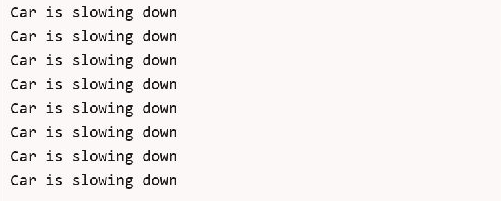
\includegraphics[width=0.62\textwidth]{figures/task1_uart.png}
\caption{UART notifications generated by B1 presses.}
\label{fig:task1-uart}
\end{figure}

\clearpage
\subsection{Implementation}
Listing~\ref{lst:task1} contains the two tasks, their creation, and the external interrupt callback. Thread flags connect the interrupt, brake action, and notification.
\lstinputlisting[caption={Task 1: priority-based brake indication and messaging.},label={lst:task1}]{../Firmware/Lab3/Lab3/Src/task1.c}

\clearpage
\section{Task 2: UART Commands, Queues, and Memory}
The UART task receives an eleven-byte frame through \texttt{HAL\_UART\_Receive\_IT}. The completion callback sets a thread flag; the task then echoes the frame and processes it. For \texttt{-DELAY 1000}, characters 2--6 identify \texttt{DELAY}, and characters 8--11 give the decimal interval. The parsed \texttt{uint16\_t} value is sent to queue 1.

The LED task waits on queue 1 with a timeout equal to the time remaining until the next toggle. A new command updates the interval and generates 150 random integers in a local array. The task scans the array and sends its maximum through queue 3. On each timeout it toggles LD2. Every ten toggles, it increments a cumulative counter and sends that value through queue 2. Queue updates notify the UART task, which prints the received values.

\subsection{Queue and Stack Allocation}
\begin{table}[H]
\centering
\caption{The three application queues, each with capacity for four items.}
\label{tab:queues}
\begin{tabular}{@{}llrrl@{}}
\toprule
Queue & Item type & Width (bytes) & Payload (bytes) & Direction \\
\midrule
1: interval & \texttt{uint16\_t} & 2 & 8 & UART $\rightarrow$ LED \\
2: count & \texttt{uint32\_t} & 4 & 16 & LED $\rightarrow$ UART \\
3: maximum & \texttt{int} & 4 & 16 & LED $\rightarrow$ UART \\
\bottomrule
\end{tabular}
\end{table}

Four items allow several pending values to be retained while the receiving task runs. Queue 1 uses the required 16-bit interval type. Queue 2 uses a 32-bit cumulative count, and queue 3 matches the array's four-byte integer type. Their combined payload is 40 bytes; FreeRTOS also allocates queue control structures from the 8192-byte heap using \texttt{heap\_4}.

The local array occupies $150\times4=600$ bytes. The LED task receives a 1536-byte stack, equivalent to 384 words, for the array, local variables, function calls, and saved context. Its measured minimum unused stack was 192 bytes, corresponding to a maximum observed use of 1344 bytes. The UART task receives a 1024-byte stack and Above Normal priority; the LED task uses Normal priority. This lets completed UART frames and queue results be processed promptly.

\subsection{Serial Results}
Figure~\ref{fig:task2-uart} shows commands echoed by the board and the subsequent queue values. Changing the interval produces a new maximum, while the toggle-group counter continues to increase. Leading zeros in \texttt{0250} are retained in the echo and converted to the integer 250 for queue 1.
\begin{figure}[H]
\centering
\begin{minipage}[t]{0.47\textwidth}
\centering
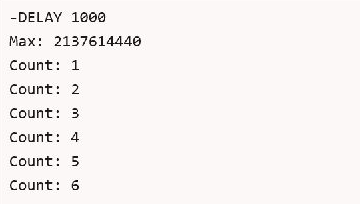
\includegraphics[width=\linewidth]{figures/task2_uart_1000.png}\\[-1mm]
\small (a) 1000 ms command
\end{minipage}\hfill
\begin{minipage}[t]{0.47\textwidth}
\centering
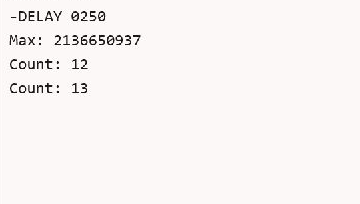
\includegraphics[width=\linewidth]{figures/task2_uart_0250.png}\\[-1mm]
\small (b) 250 ms command
\end{minipage}
\caption{Task 2 output: command echo, array maximum, and cumulative count.}
\label{fig:task2-uart}
\end{figure}

\clearpage
\subsection{Implementation}
The UART task is the sole owner of serial transmission. It rearms reception after consuming the completed frame and drains queues 2 and 3 when notified.
\lstinputlisting[firstline=1,lastline=69,caption={Task 2: command parsing and UART task.},label={lst:uart}]{../Firmware/Lab3/Lab3/Src/task2.c}

\clearpage
The LED task maintains an absolute deadline between toggles. Queue reception can wake it before that deadline to apply a new interval and generate the array. The stack allocation and queue widths are set when the application starts.
\lstinputlisting[firstline=71,lastline=144,firstnumber=71,caption={Task 2: LED task, queue creation, and receive callback.},label={lst:led}]{../Firmware/Lab3/Lab3/Src/task2.c}

\clearpage
\subsection{Measured LED Timing}
PA5 output states were sampled through ST-LINK while the application ran. Twelve successive transitions were recorded for each command, giving eleven inter-toggle intervals. Figure~\ref{fig:timing} shows the first 3.2 s of each trace, and Table~\ref{tab:timing} summarizes the intervals.

\begin{figure}[H]
\centering
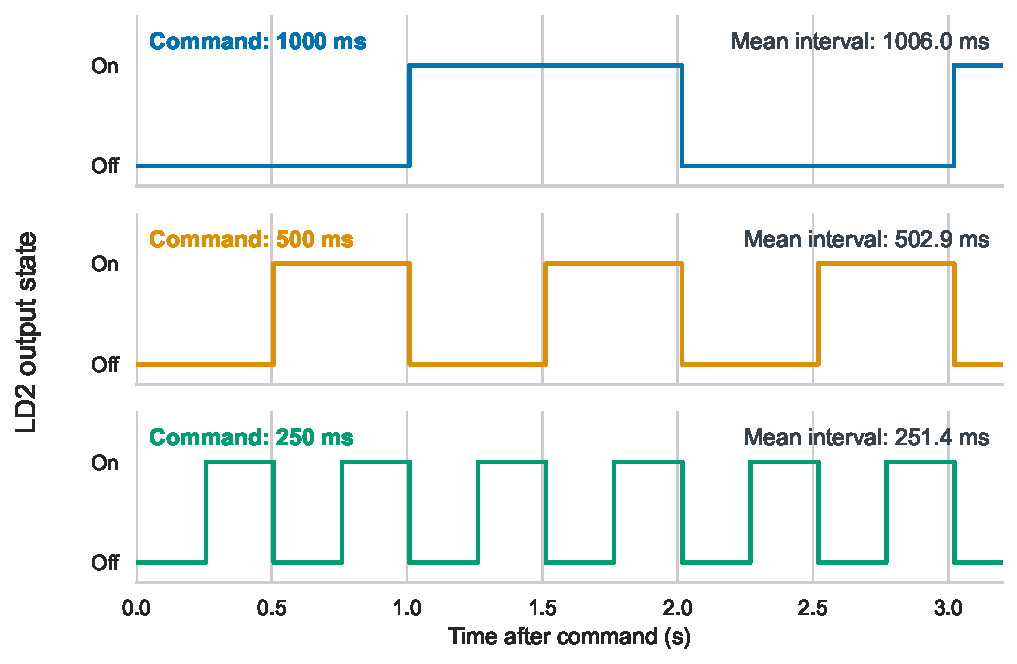
\includegraphics[width=\textwidth]{figures/led_timing.pdf}
\caption{Recorded LD2 output states for three commanded toggle intervals.}
\label{fig:timing}
\end{figure}

\begin{table}[H]
\centering
\caption{Measured inter-toggle intervals. SD denotes sample standard deviation.}
\label{tab:timing}
\begin{tabular}{@{}rrrr@{}}
\toprule
Command (ms) & Mean (ms) & SD (ms) & Intervals \\
\midrule
1000 & 1006.0 & 0.9 & 11 \\
500 & 502.9 & 0.7 & 11 \\
250 & 251.4 & 0.8 & 11 \\
\bottomrule
\end{tabular}

\end{table}

The mean interval scales with the requested delay and is approximately 0.6\% above the nominal value in each case. A complete on/off cycle contains two toggles, so its period is $2T$. The counter is updated every ten toggles, corresponding to nominal update periods of 10, 5, and 2.5 s for the three commands.

\section{Conclusion}
The first task demonstrated priority-based response by applying the brake indicator before issuing its UART notification. The second task combined interrupt-driven reception with three queues to control LED timing and report counter and array results. Hardware output confirmed command parsing and queue communication, while measured intervals followed the requested 4:2:1 ratio. Allocating 1536 bytes to the LED task accommodated the 600-byte local array and its execution stack.
\end{document}
